\documentclass[a4paper,11pt]{article}

\usepackage[T1]{fontenc}
\usepackage[polish]{babel}
\usepackage[utf8]{inputenc}
\usepackage{lmodern}
\selectlanguage{polish}
\usepackage[top=2cm, bottom=2cm, left=3cm, right=3cm]{geometry}

\makeatletter
\newcommand{\linia}{\rule{\linewidth}{0.4mm}}
\renewcommand{\maketitle}{\begin{titlepage}
    \vspace*{2cm}
    \begin{center}\LARGE
    Politechnika Warszawska\\
    Wydział Elektryczny\\
    \end{center}
    \vspace{5cm}
    \noindent\linia
    \begin{center}
      \LARGE \textsc{\@title}
         \end{center}
     \linia
    \vspace{0.5cm}
    \begin{flushright}
    \begin{minipage}{5cm}
    \textit{Autorzy:}\\
    \normalsize \textsc{\@author} \par
    \end{minipage}
    \vspace{5cm}
     \end{flushright}
    \vspace*{\stretch{6}}
    \begin{center}
    \@date
    \end{center}
  \end{titlepage}%
}
\makeatother
\author{Grzegorz Kopyt\\
Daniel Sporysz}
\title{Sprawozdanie\\
,,WireWorld''}

\usepackage{graphicx}
\begin{document}

\maketitle


\tableofcontents
\vspace{1cm}
\noindent\linia



\section{Opis działania}
Program jest implementacją automatu komórkowego opartego na regułach ,,gry w życie'' Johna Conwaya w wariancie ,,WireWorld''.

Za pomocą interfejsu graficznego program przedstawia zmiany pól jakie zachodzą na planszy zgodnie z zasadami gry.

Pracę programu można konfigurować na kilka sposobów: wczytać początkową konfigurację planszy z pliku graficznego, stworzyć własną planszę za pomocą narzędzi do edycji pól lub w sposób mieszany, czyli wczytując konfigurację z pliku i dalsza jego edycja za pomocą edytora programu.

Analizę i modyfikację planszy można przerwać lub wznowić w każdej chwili pracy programu. Gdy generacja jest wstrzymana, użytkownik może ręcznie zmodyfikować planszę lub zapisać jej obecny stan do pliku graficznego.

\noindent\linia
\section{Możliwości programu}


\subsection{Edycja planszy}
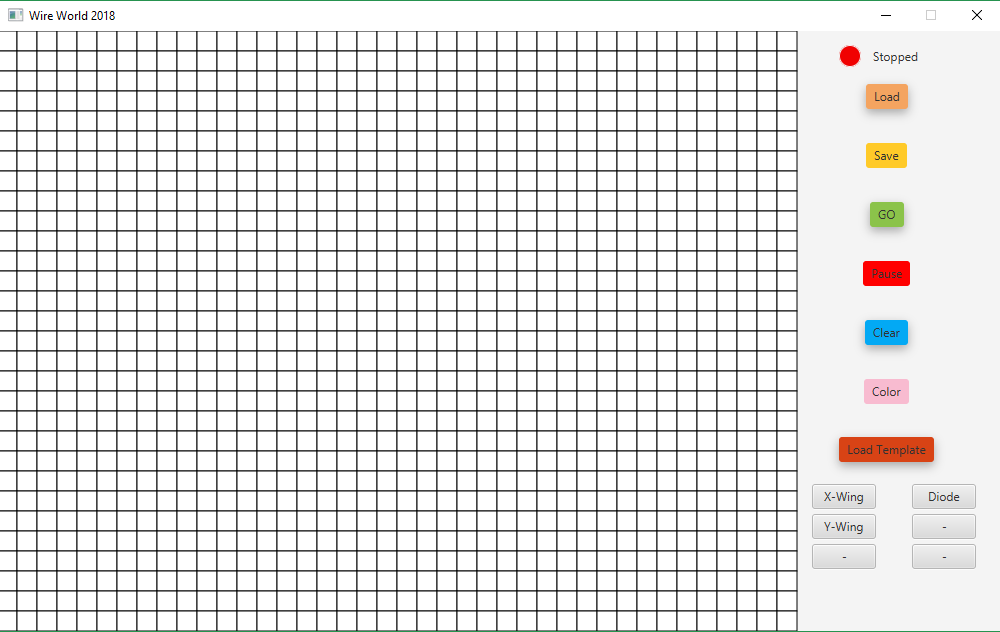
\includegraphics[width=\textwidth]{mainScreen}
\begin{itemize}
\item Zmiana koloru pól poprzez "przeciągnięcie'' - zmieniają się w kolejności pusty->przewodnik->ogon->głowa.
\item Zmiana koloru pól poprzez ''kliknięcie'' lewym przyciskiem myszy - zmieniają się w kolejności pusty->przewodnik->ogon->głowa.
\item Zmiana koloru pól poprzez ''kliknięcie'' prawym przyciskiem myszy - nadanie koloru pusty.
\item Wstawianie gotowych wzorów na plansze poprzez naciśnięcie jednego z przycisków w prawym dolnym rogu i przesuwając kursorem na planszy umieszczenie go w wybranym miejscu i zatwierdzenie lewym przyciskiem myszy lub porzucenie prawym (możliwość obrotu elementów poprzez ''scroll").

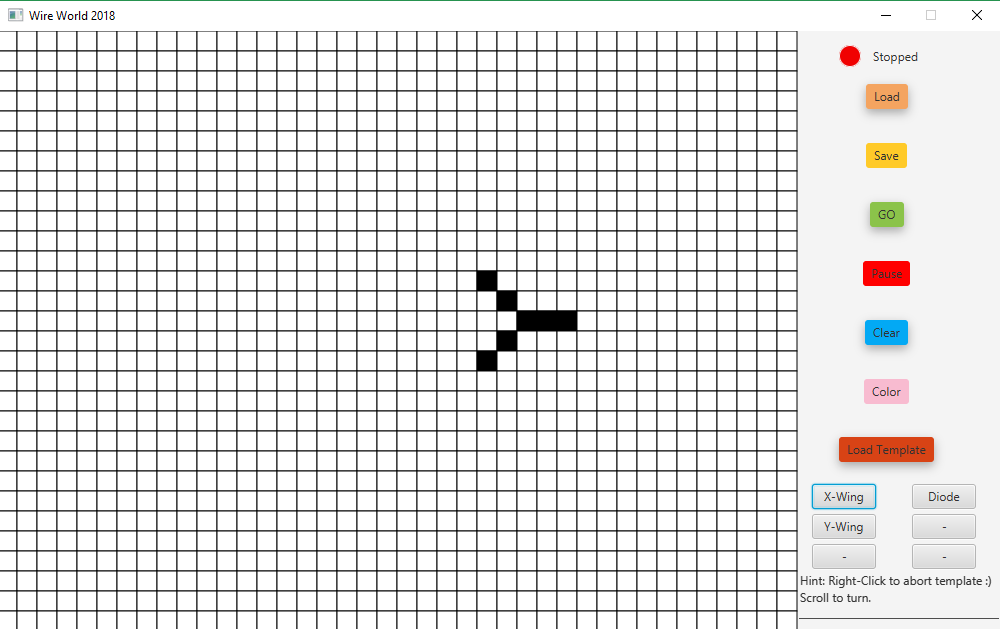
\includegraphics[width=\textwidth]{insertTemplate}
 
\end{itemize}
\subsection{ Zmiana domyślnych kolorów planszy}
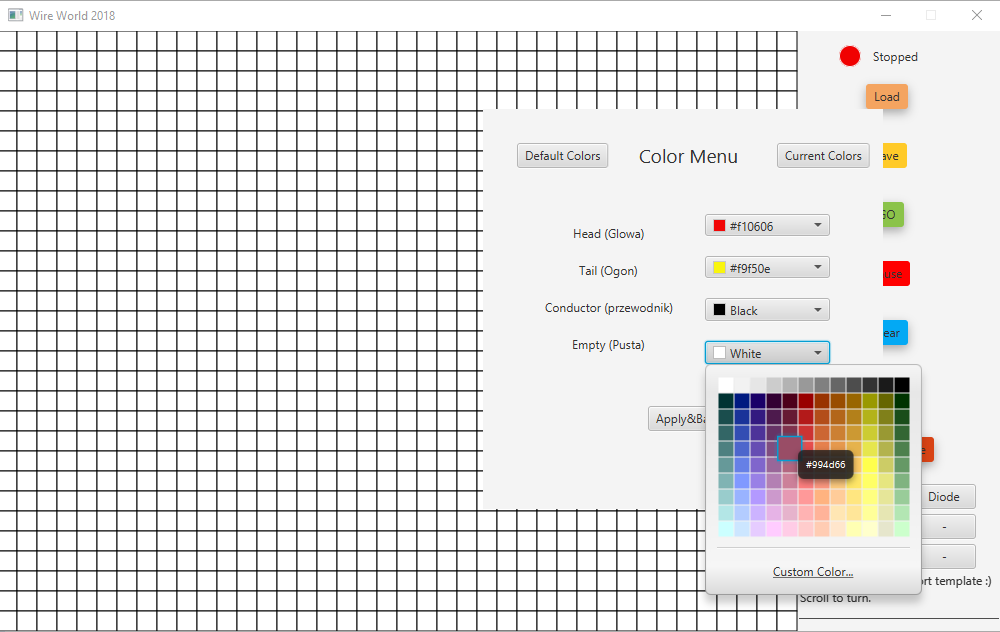
\includegraphics[width=\textwidth]{colorMenu}
\begin{itemize}
\item W wygodnym meny koloru można wybrać własne kompozycje kolorów.
\end{itemize}
\subsection{Dodawanie własnych wzorów}
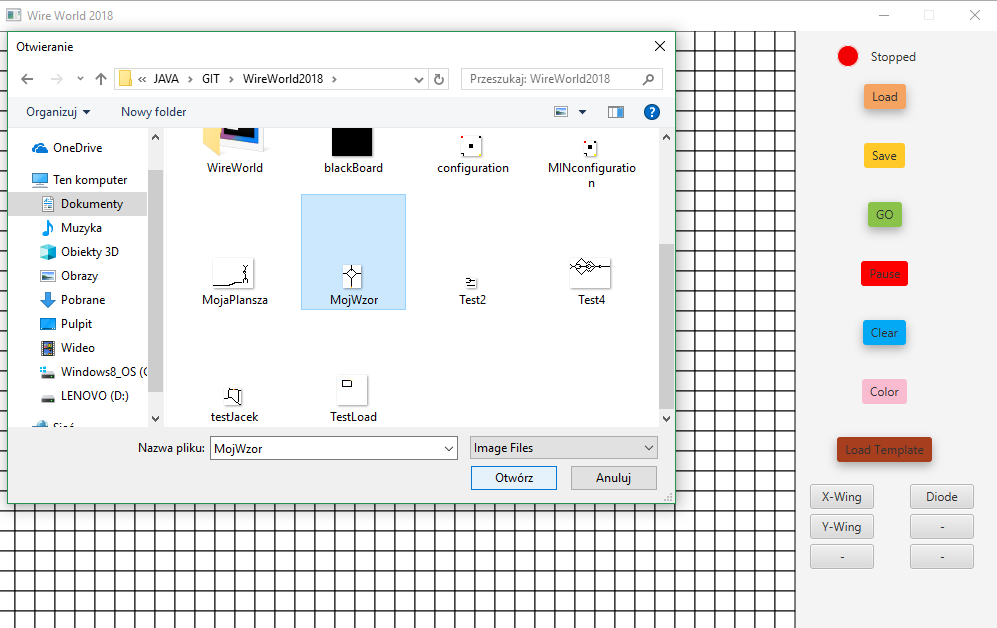
\includegraphics[width=\textwidth]{addWzor1}

\begin{itemize}
\item Możliwość dodania trzech wzorów poprzez przycisk ''LoadTemplate''
\item Nazwa pliku ze wzorem pojawi się na jednym z przycisków w prawym dolnym rogu.

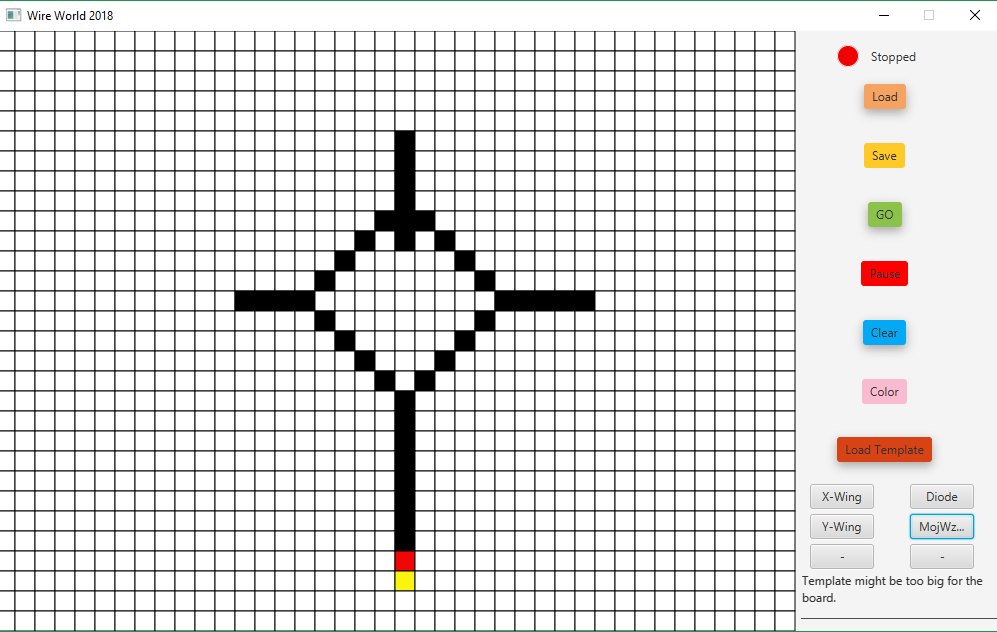
\includegraphics[width=\textwidth]{addWzor2}
\item Plik musi być w formacie graficznym (.png, .jpeg), pokolorowany kolorami biały(pusty), czarny(przewodnik), żółty(ogon), czerwony(głowa)
\end{itemize}

\subsection{Zapis planszy do pliku}
\begin{itemize}
\item Przycisk ''Save'' prowadzi do menu zapisu, gdzie mamy możliwość wyboru nazwy i lokalizacji pliku

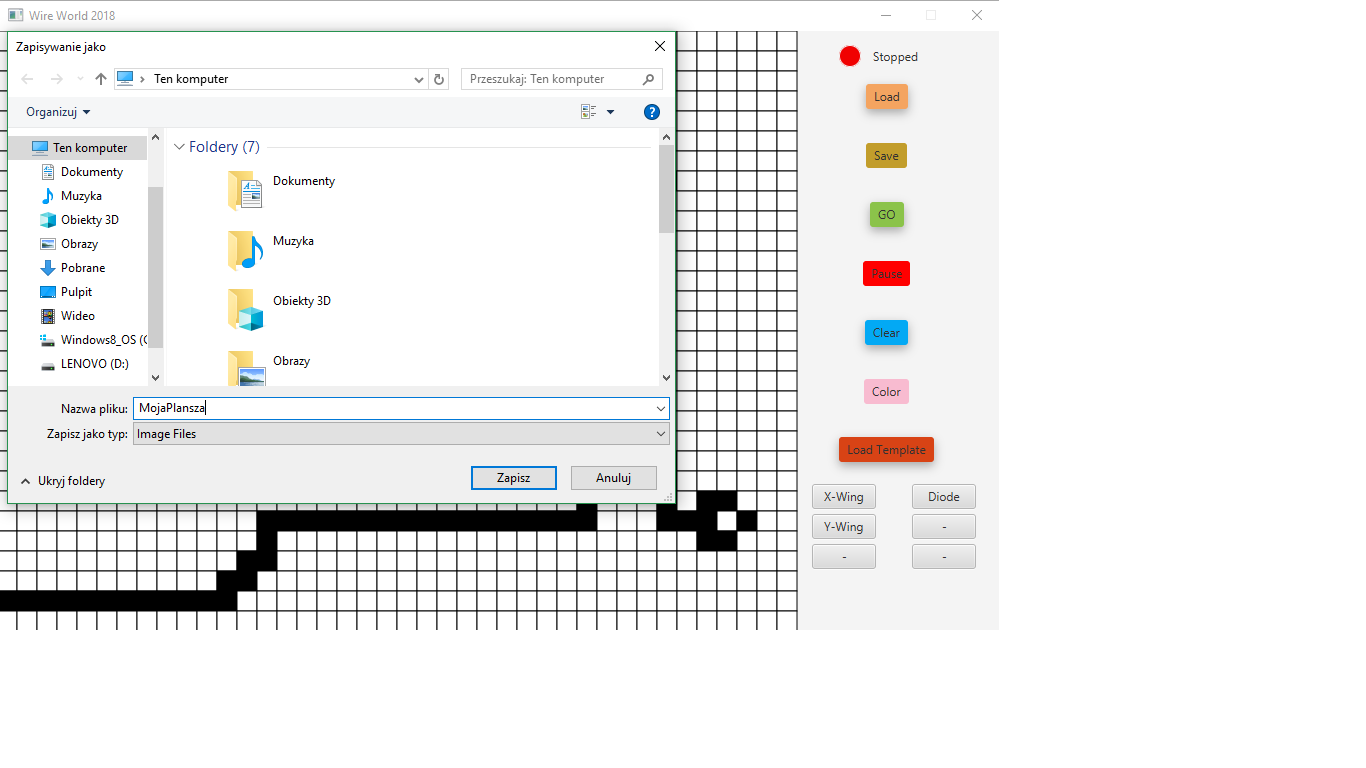
\includegraphics[width=\textwidth]{zapis}
\end{itemize}

\subsection{Wczytanie planszy z pliku}
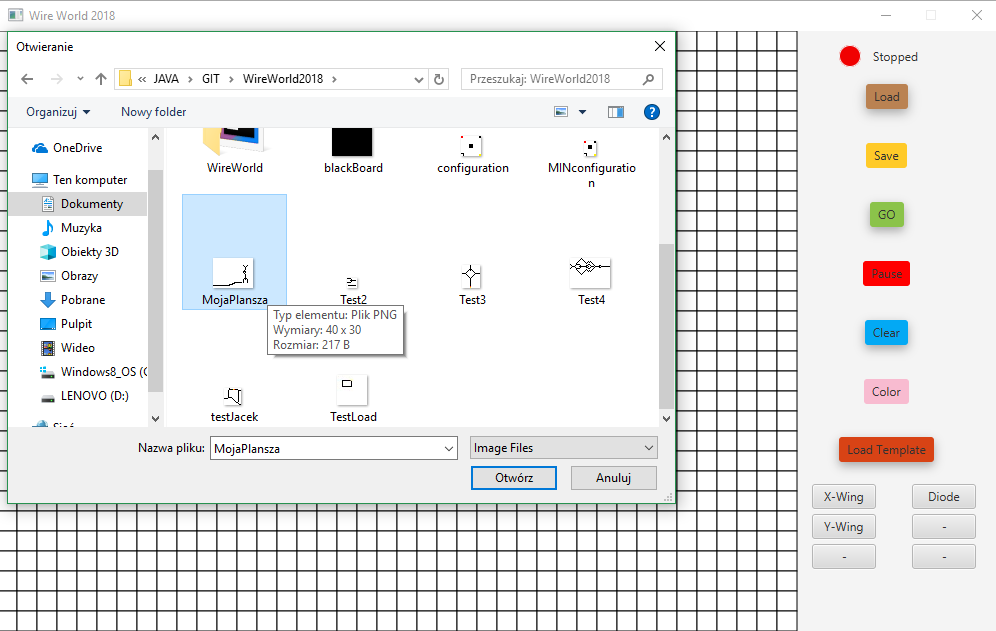
\includegraphics[width=\textwidth]{load}
\begin{itemize}
\item Przycisk 'Load'' prowadzi do menu wyboru plików, gdzie mamy możliwość odnalezienia nazwy i lokalizacji pliku
\item Plik zostaje wczytany i  od razu nałożony na plansze
\end{itemize}

\subsection{Animacja}
\begin{itemize}
\item Klatka 1 przykładowej konfiguracji planszy
\end{itemize}
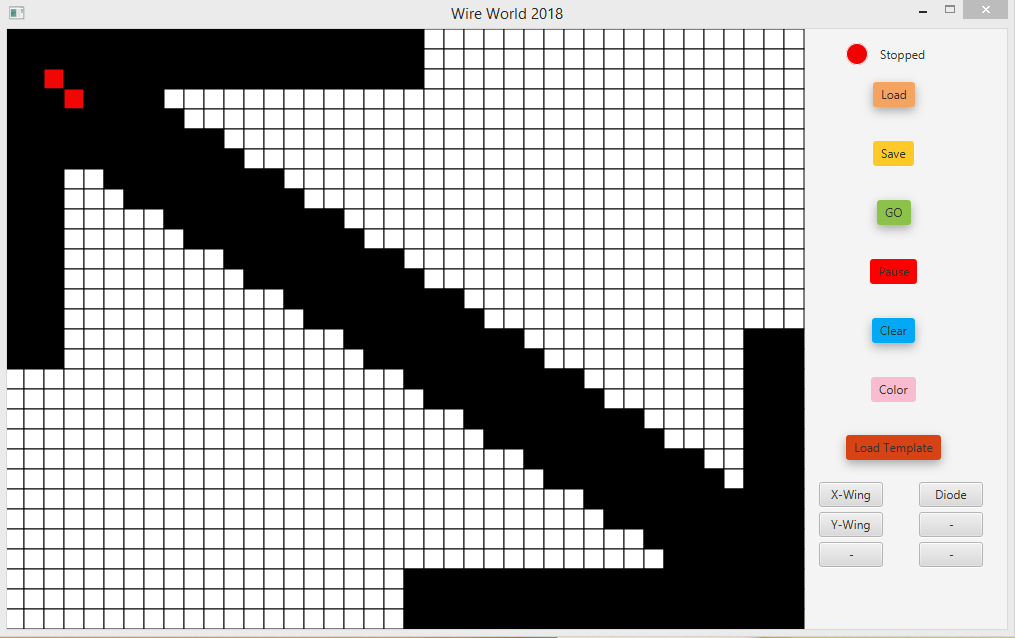
\includegraphics[width=\textwidth]{GenFrame1}
\begin{itemize}
\item Klatka 2 przykładowej konfiguracji planszy
\end{itemize}
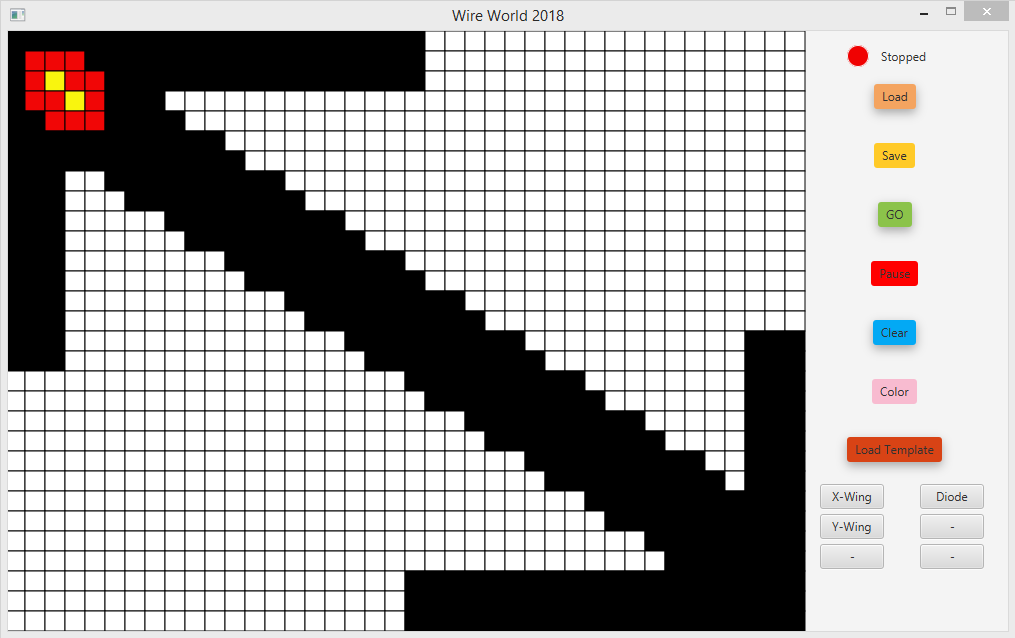
\includegraphics[width=\textwidth]{GenFrame2}
\begin{itemize}
\item Klatka n-ta przykładowej konfiguracji planszy
\end{itemize}
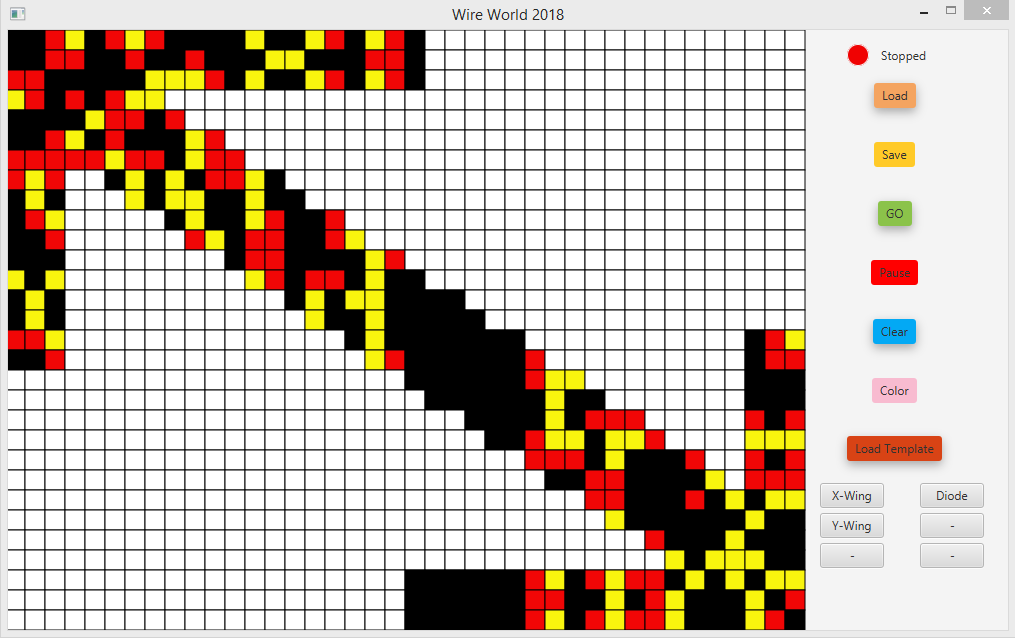
\includegraphics[width=\textwidth]{GenFrame69}
\begin{itemize}
\item Powyższe zrzuty ekranu z pracy aplikacji ukazują pracę generatora nowych klatek wspieranego przez interfejs graficzny. 
\item Powyższy przykład ukazuje również jaki jest domyślny sposób analizy planszy, czyli analizowanie planszy w trybie ,,bez ramkowym'', czyli komórki na granicach planszy wchodzą w interakcję z tymi po ,,drugiej stronie ekranu''.
\item Zrzuty ekranu zostały wykonane przy domyślnym motywie kolorów reprezentujących stany komórek.
\end{itemize}

\noindent\linia
\section{Opis implementacji}

\subsection{Implementacja modułu ,,Board''}

\begin{enumerate}
\item Wprowadzono klasę Cell rozszerzającą Rectangle, aby móc wyodrębnić w niej metodę zmieniającą kolor, a także pola współrzędnych na planszy danej komórki oraz pole "poprzedniego koloru". Porządkuje to kod i ułatwia korzystanie z klasy Rectangle do naszych celów.
\item Metoda makeBoard otrzymuje dodatkowo jako argumenty wymiary obiektu Pane, na którym będzie tworzona plansza, ponieważ metody inicjujące GUI potrzebowały tej informacji
\item Dodano szereg funkcji pozwalających na kontrolę planszy:
	\begin{itemize}
	\item repaintBoard - nadaje planszy obecne kolory i ustawia "poprzednie kolory" komórek na obecne
	\item setBoardColor - nadaje całej planszy jeden kolor
	\item repaintBoardOnPrevious - maluje komórki planszy na jej poprzednie kolory
	\item setColorMode - ustawia tryb planszy na zwykłe kolorowanie planszy poprzez "kliknięcia" i "przeciągnięcia"
	\item setCurrentBoardMode - nadaje wartość obecnego trybu planszy
	\item setInsensitiveMode - ustawia tryb planszy, w którym jest ona nieczuła na edycje
	\item setTemplateInsertionMode - ustawia tryb planszy na wprowadzanie wzorów
	\end{itemize}

\item W klasie Template zdefiniowano metody wstawiania wzoru na plansze, we wszystkie cztery możliwe kierunki

\end{enumerate}


\subsection{Zmiany w implementacji modułu ,,GUI''}

\begin{enumerate}
\item Do menu wyboru kolorów dodano przycisk powrotu do domyślnych kolorów, a także przycisk ustawienia obecnych kolorów na przyciskach wyboru koloru, co ułatwia zarządzanie kolorami planszy.
\item Do kontrolerów dodano pole Colors , aby przekazywać informacje o obecnych kolorach planszy
\item MainScreenController otrzymał pole BoardMaker, aby przekazywać mu sterowanie naszą planszą
\item MainScreenControlle otrzymał szereg metod kontrolujących elementy tej sceny:
	\begin{itemize}
	\item disableNonTemplateButtons - blokuje dostęp do przycisków nie służących do wstawiania wzorów
	\item disableTemplateButtons - blokuje dostęp do przycisków służących do wstawiania wzorów
	\item isAnimationRunningSignal - pozwala na włączenie lub wyłączenie obiektu pokazującego czy animacja obecnie działa
	\item manageTemplateInsertion - porządkuje działania w metodach pod przyciskami do wstawiania wzorów
	\end{itemize}
\end{enumerate}

\subsection{Implementacja pakietu ,,Generation''}
\subsubsection{Zmiany w klasie GenerationsHandler}
\begin{enumerate}
\item Nazwa obiektu zmieniona na ,,GeneratorHandler'', aby lepiej wyrazić zastosowanie klasy.
\item Dodano nowe pole ,,running'' typu boolean na potrzeby cechy wielowątkowości programu
\item Dodano dwie metody set i get dla pola ,,mode''
\item Dodano nowe pole ,,generator'' typu Generation.CellularAutomation
\item Dodano funkcję ,,terminate'', która wstrzymuje pracę generatora ostatecznie, co pozwala na przerwanie pracy wątku generatora
\end{enumerate}
\subsubsection{Dodano klasę StatusIndicators}
\begin{enumerate}
\item Klasa ta zawiera nazwy stałych ( String ) i ich wartości ( int ), określające stany w których mogą się znajdować komórki planszy. tj.:
\begin{enumerate}
\item HEAD = 3
\item TAIL = 2
\item CONDUCTOR = 1
\item EMPTY = 0
\end{enumerate}
\item Klasa zapewnia lepszą czytelność kodu dla innych klas z pakietu
\end{enumerate}
\subsubsection{Zmiany w klasie CellularAutomation}
\begin{enumerate}
\item Dodano pole ,,adapter'' typu Generation.BoardAdapter ułatwiający i standaryzujący dostęp do pól analizowanej planszy
\item Zrezygnowano z pól ,,headColor'', ,,tailColor'', ,,conductorColor'' oraz ,,emptyFieldColor'', które nie znalazły zastosowania w tej klasie
\item Dodano metodę ,,updateBoard'', która na podstawie informacji zawartych w polu ,,tmpMatrix'' uaktualnia stany komórek na planszy
\item Dodano metodę ,,setBorderss'', która służy rolę przekaźnika instrukcji do obiektu ,,Neighbours''
\end{enumerate}
\subsubsection{Dodano klasę BoardAdapter}
\begin{enumerate}
\item Obiekt ten zawiera pola ,,list'' (ArrayList<Cell>), ,,height'' (int) i ,,width'' (int), które opisują oraz zawierają informacje o planszy komórek
\item Klasa ta zapełnia łatwiejszy dostęp do komórek planszy
\item Obecność klasy zwalnia pozostałe obiekty z wiedzy w jaki sposób komórki są przechowywane w pamięci
\end{enumerate}
\subsubsection{Zmiany w klasie Rules}
\begin{enumerate}
\item W instrukcjach warunkowych oraz przy wyrażaniu wartości zwracanych wykorzystano stałe z obiektu Generation.StatusIndicators, co przełożyło się na lepsza czytelność kodu oraz jego łatwiejsze zrozumienie.
\item Brak zmian w strukturze oraz logice pracy obiektu
\end{enumerate}
\subsubsection{Zmiany w klasie Rules}
\begin{enumerate}
\item Zrezygnowano z pola ,,rectangleMap'' typu HashMap<String, javafx.scene.shape.Rectangle> na rzecz pola ,,adapter'' Generation.BoardAdapter
\item Dodano pole ,,adapter'' typu Generation.BoardAdapter ułatwiający i standaryzujący dostęp do pól analizowanej planszy
\item W wyniku analizy pracy programu dostrzeżono wspólne zachowanie dwóch funkcji ,,neighbours'' i ,,borderlessNeighbours''. W wyniku czego została wyodrębniona nowa metoda ,,analyzeCell'', która sprawdza czy komórka o podanym indeksie znajduje się na planszy oraz w przypadku, gdy pytana komórka jest w stanie ,,3'' - zwiększa licznik ,,heads''
\end{enumerate}

\subsection{Implementacja pakietu ,,IO''}
\subsubsection{Zmiany w klasie IO}
\begin{enumerate}
\item xxxxxxxxxxxxxxx
\end{enumerate}


\noindent\linia
\section{Opcje rozbudowy programu}
\begin{enumerate}

\item Pakiet Generation został zaprojektowany do pracy z planszą o dowolnych rozmiarach, co oznacza, że możliwa jest stosunkowa szybka i prosta modyfikacja programu do pracy na różnych wymiarach planszy.

\item Pakiet Generation wspiera funkcję przełączania trybu analizy planszy pomiędzy trybami ,,z granicami'' oraz ,,bez granic''.

\item Pakiet Generation wspiera opcję ustawienia szybkości generowania kolejnych klatek ukazujących stany komórek na planszy.

\end{enumerate}
\end{document}



